\begin{savequote}[8cm]
\begin{CJK*}{UTF8}{min}
おれは海賊王になる男だ!!!
\end{CJK*}

I'll be the one to measure $\dcp$.
  \qauthor{--- Monkey D. Luffy}
\end{savequote}

\chapter{\label{ch:t2k}The T2K Experiment} 

\minitoc
The T2K experiment is a long-baseline neutrino experiment with the aim of measuring CP violation in the lepton sector through neutrino oscillation measurements.  
This chapter begins by describing the experimental setup and then provides a concise overview of the software, thereby laying the groundwork for the subsequent analyses.

\section{Hardware}
As a long-baseline experiment, T2K encompasses a near detector (ND280) and a far detector (Super-Kamiokande, often referred to as Super-K).  
Both detectors must discriminate between \(\numu\) and \(\nue\) to measure neutrino oscillations.  
Naturally, detecting neutrinos directly is impossible.  
Instead, each detector must be able to identify the different particles produced when neutrinos interact with its active material.  
Most commonly, such neutrino–nucleus interactions generate the corresponding leptons (i.e., electrons or muons) and various hadrons, including protons, neutrons, and light mesons such as pions.

The far detector, SK, is a large water Cherenkov detector.  
It detects particles by collecting the Cherenkov light emitted when they travel faster than the speed of light in water.  
Hadrons resulting from neutrino interactions typically lack sufficient energy to emit Cherenkov radiation, whereas leptons often exceed this threshold.  
Consequently, SK primarily observes electrons and muons, whose Cherenkov radiation forms ring-like patterns transverse to their direction of flight.  
Because the electron is lighter than the muon, its path is more prone to scattering, causing the electron’s Cherenkov ring to appear more diffuse than the muon’s, as illustrated in Fig.~\ref{fig:sk-e-mu}.

\begin{figure}
    \centering
    \begin{subfigure}[b]{\dbfigwid\textwidth}
        \centering
        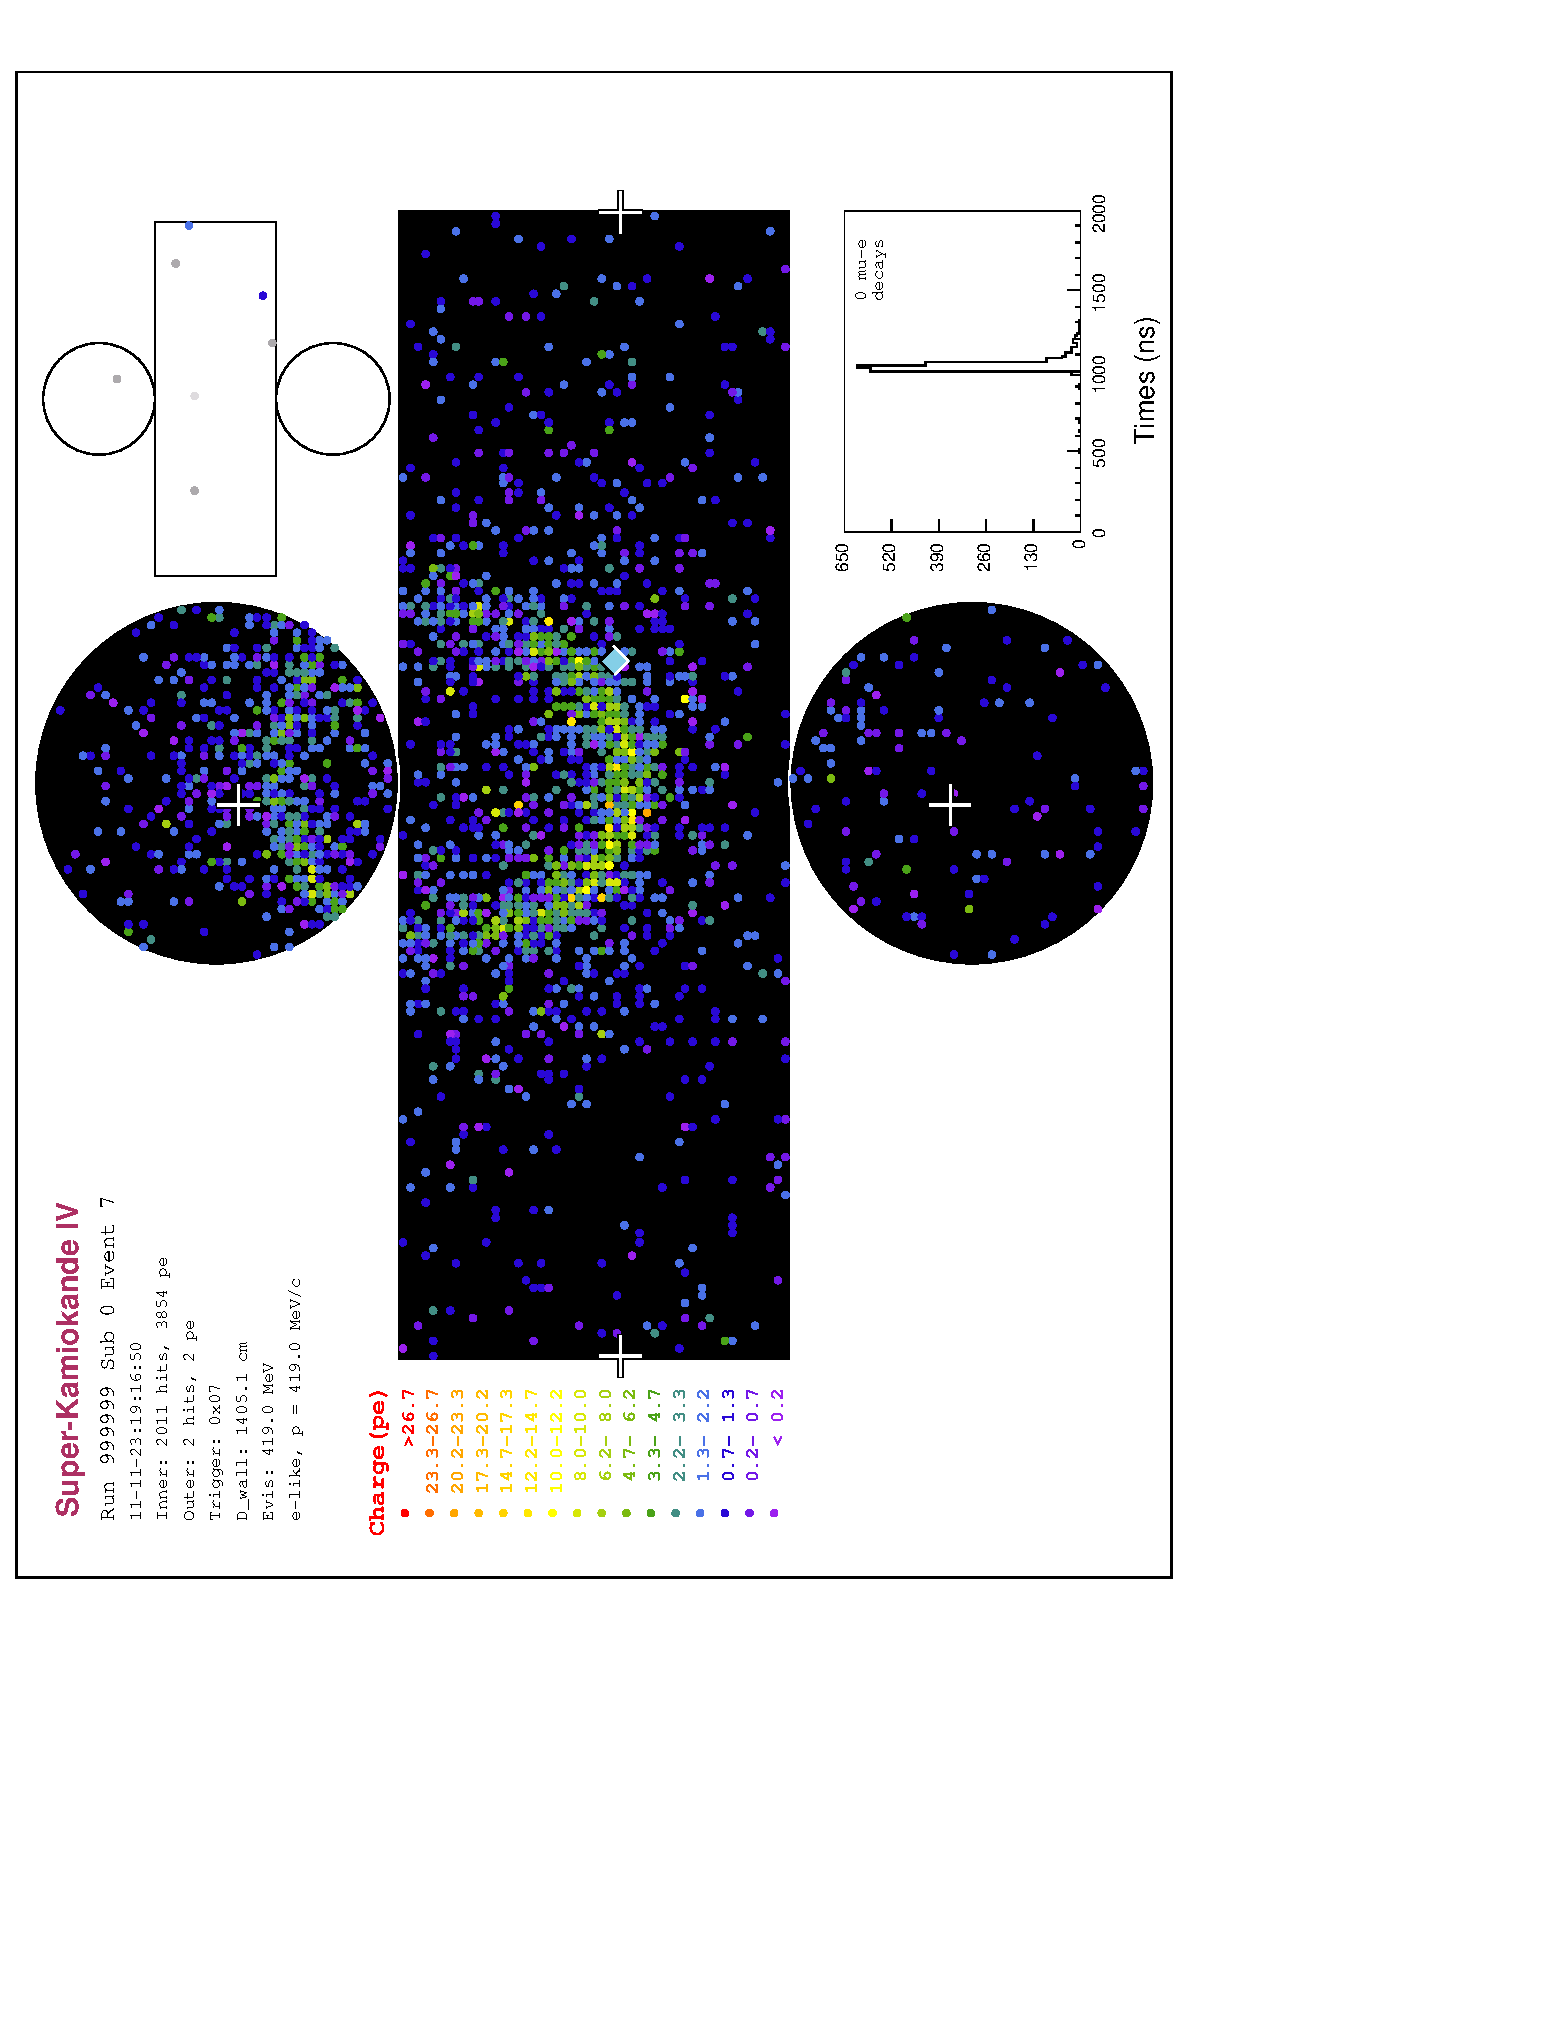
\includegraphics[width=\textwidth]{figures/t2k/sk-nue.eps}
        \caption{\(\nu_e\)}
        \label{subfig:sk-nue}
    \end{subfigure}
    \begin{subfigure}[b]{\dbfigwid\textwidth}
        \centering
        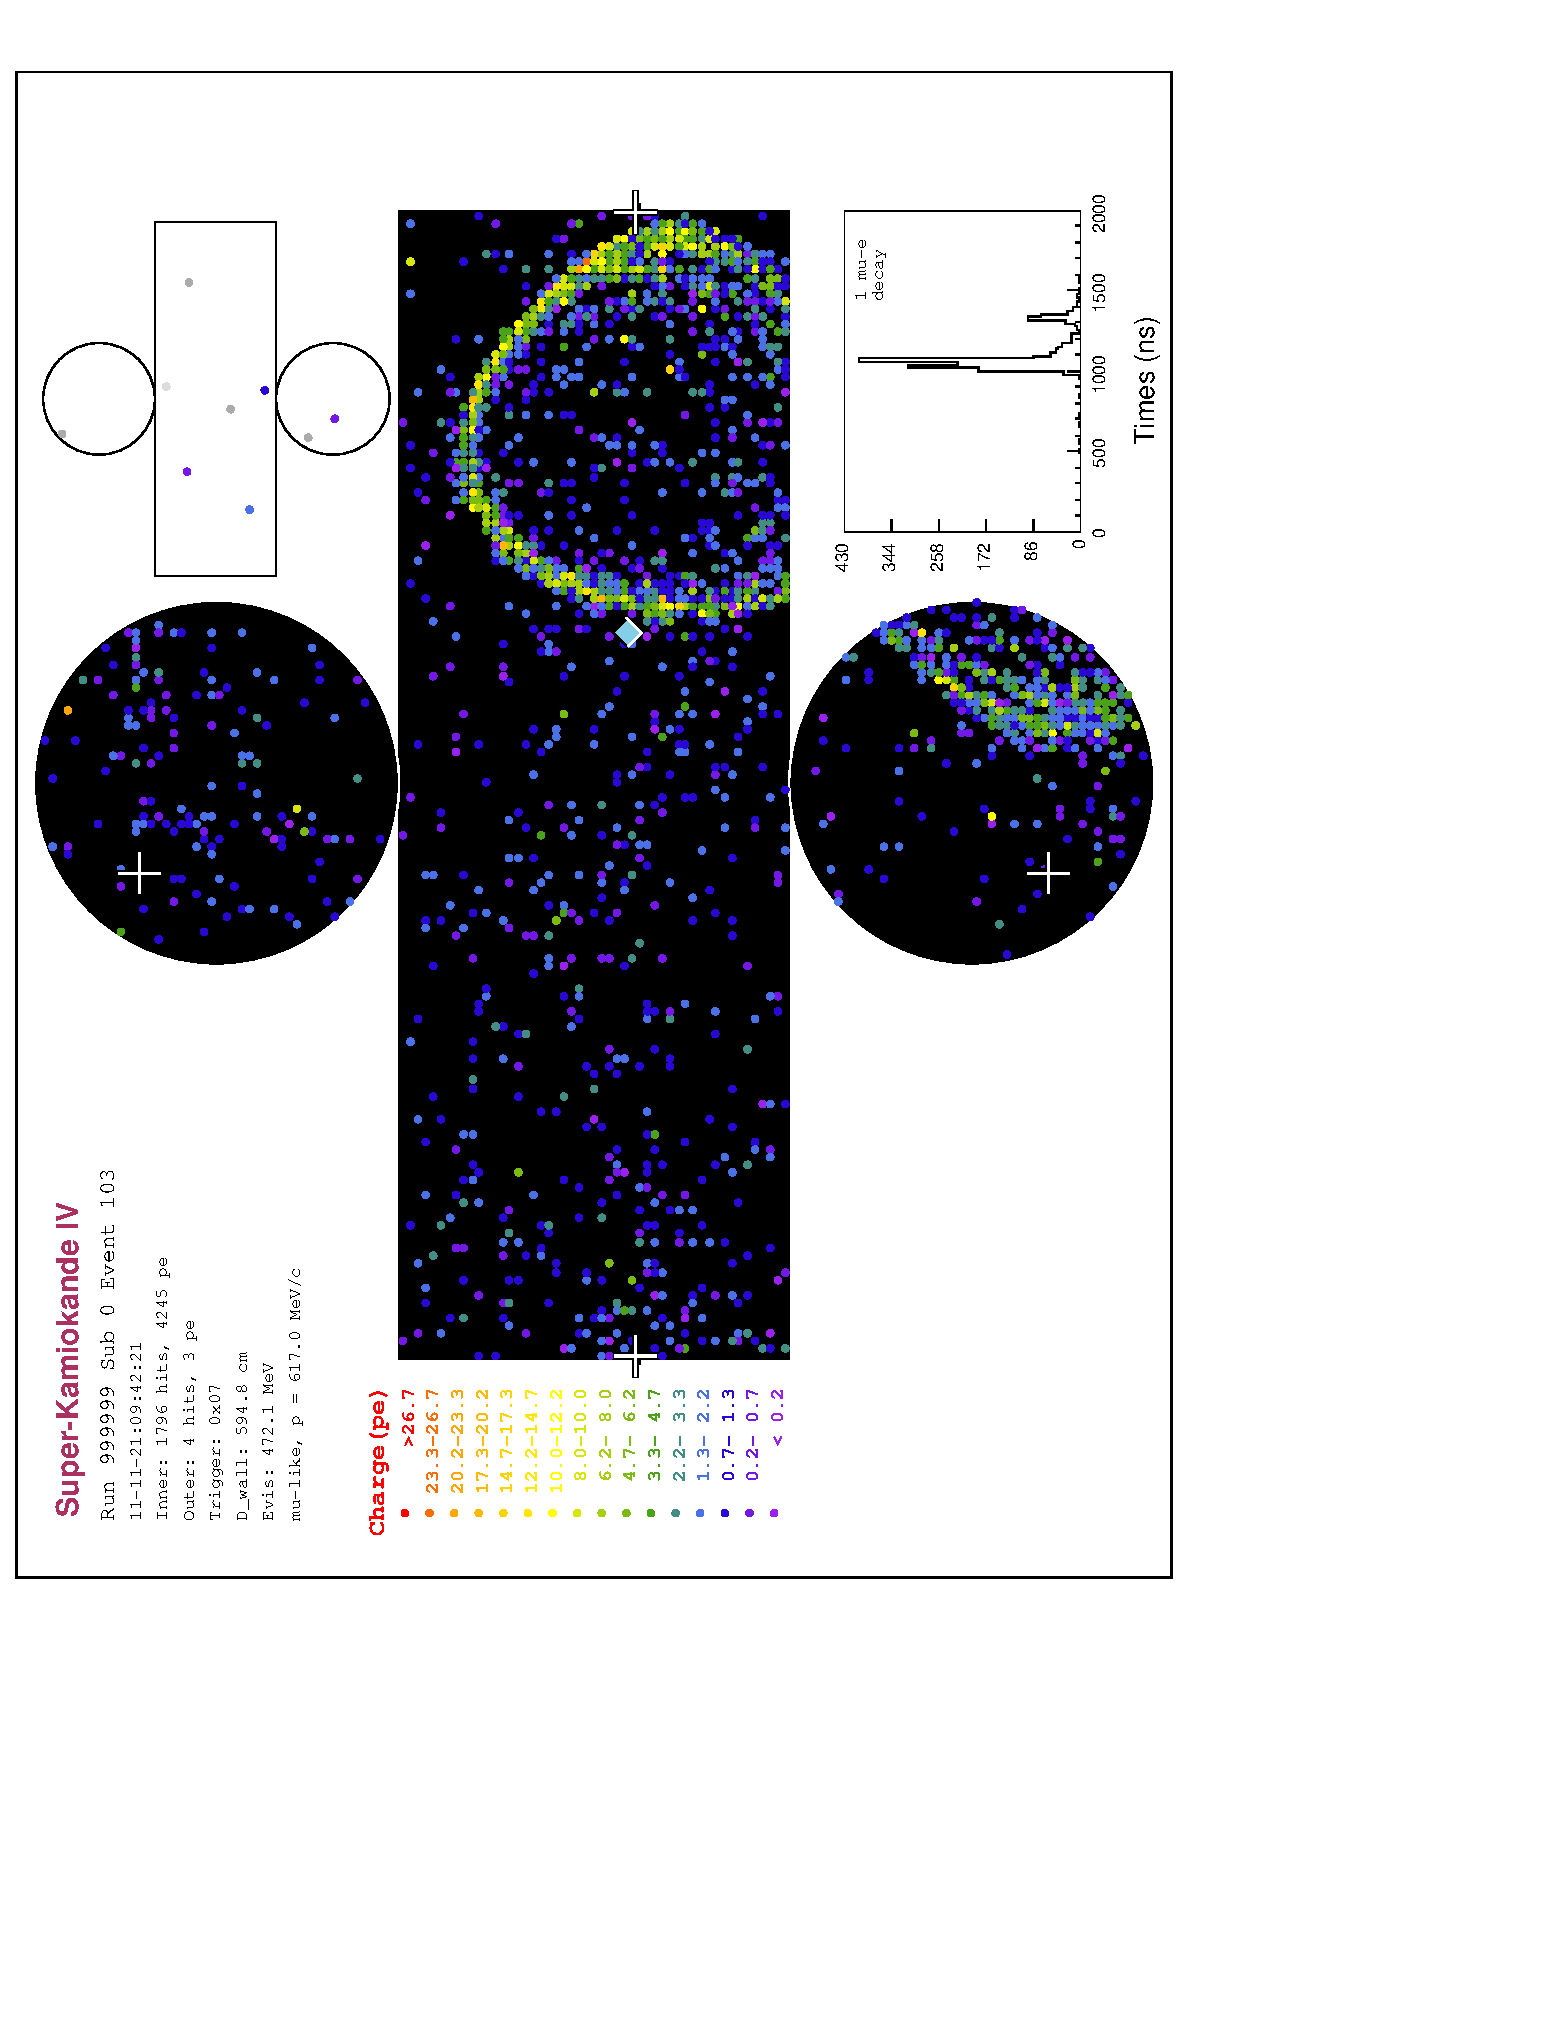
\includegraphics[width=\textwidth]{figures/t2k/sk-numu.eps}
        \caption{\(\nu_\mu\)}
        \label{subfig:sk-numu}
    \end{subfigure}
    \caption{SK event displays.}
    \label{fig:sk-e-mu}
\end{figure}

In contrast, the near detector, ND280, consists of multiple specialized subdetectors designed to measure as many neutrino interaction products as well as possible.  
The classic ND280 configuration is shown in Fig.~\ref{subfig:nd280-classic}.  
Its central detector assembly contains a \(\piz\)-detector (P0D), three vertical Time Projection Chambers (TPCs), and two Fine Grained Detectors (FGDs) positioned between the TPCs.  
Surrounding these devices are various electromagnetic calorimeters (ECALs)—the P0D ECAL, the Barrel ECAL, the Upstream ECAL, and the Downstream ECAL—all enclosed by the UA1 magnet comprising a solenoid coil and a yoke.

\begin{figure}
    \centering
    \begin{subfigure}[b]{\dbfigwid\textwidth}
        \centering
        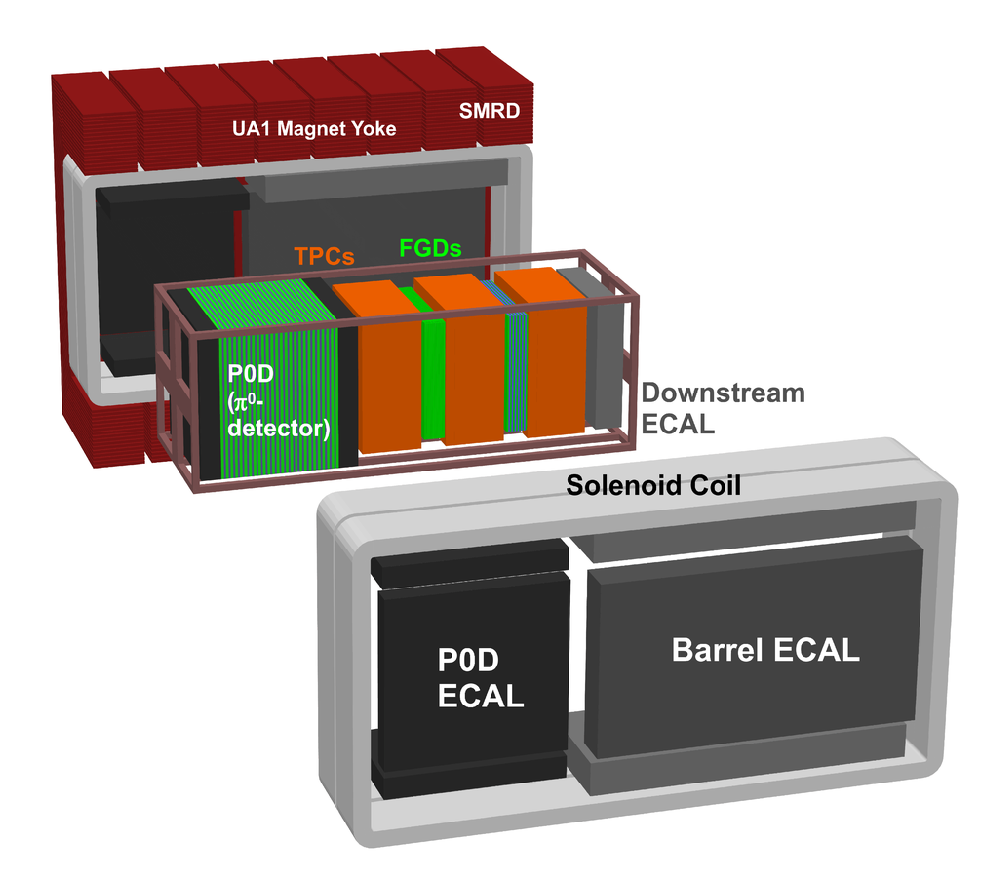
\includegraphics[width=\textwidth]{figures/t2k/ND280-classic.eps}
        \caption{Classic}
        \label{subfig:nd280-classic}
    \end{subfigure}
    \begin{subfigure}[b]{\dbfigwid\textwidth}
        \centering
        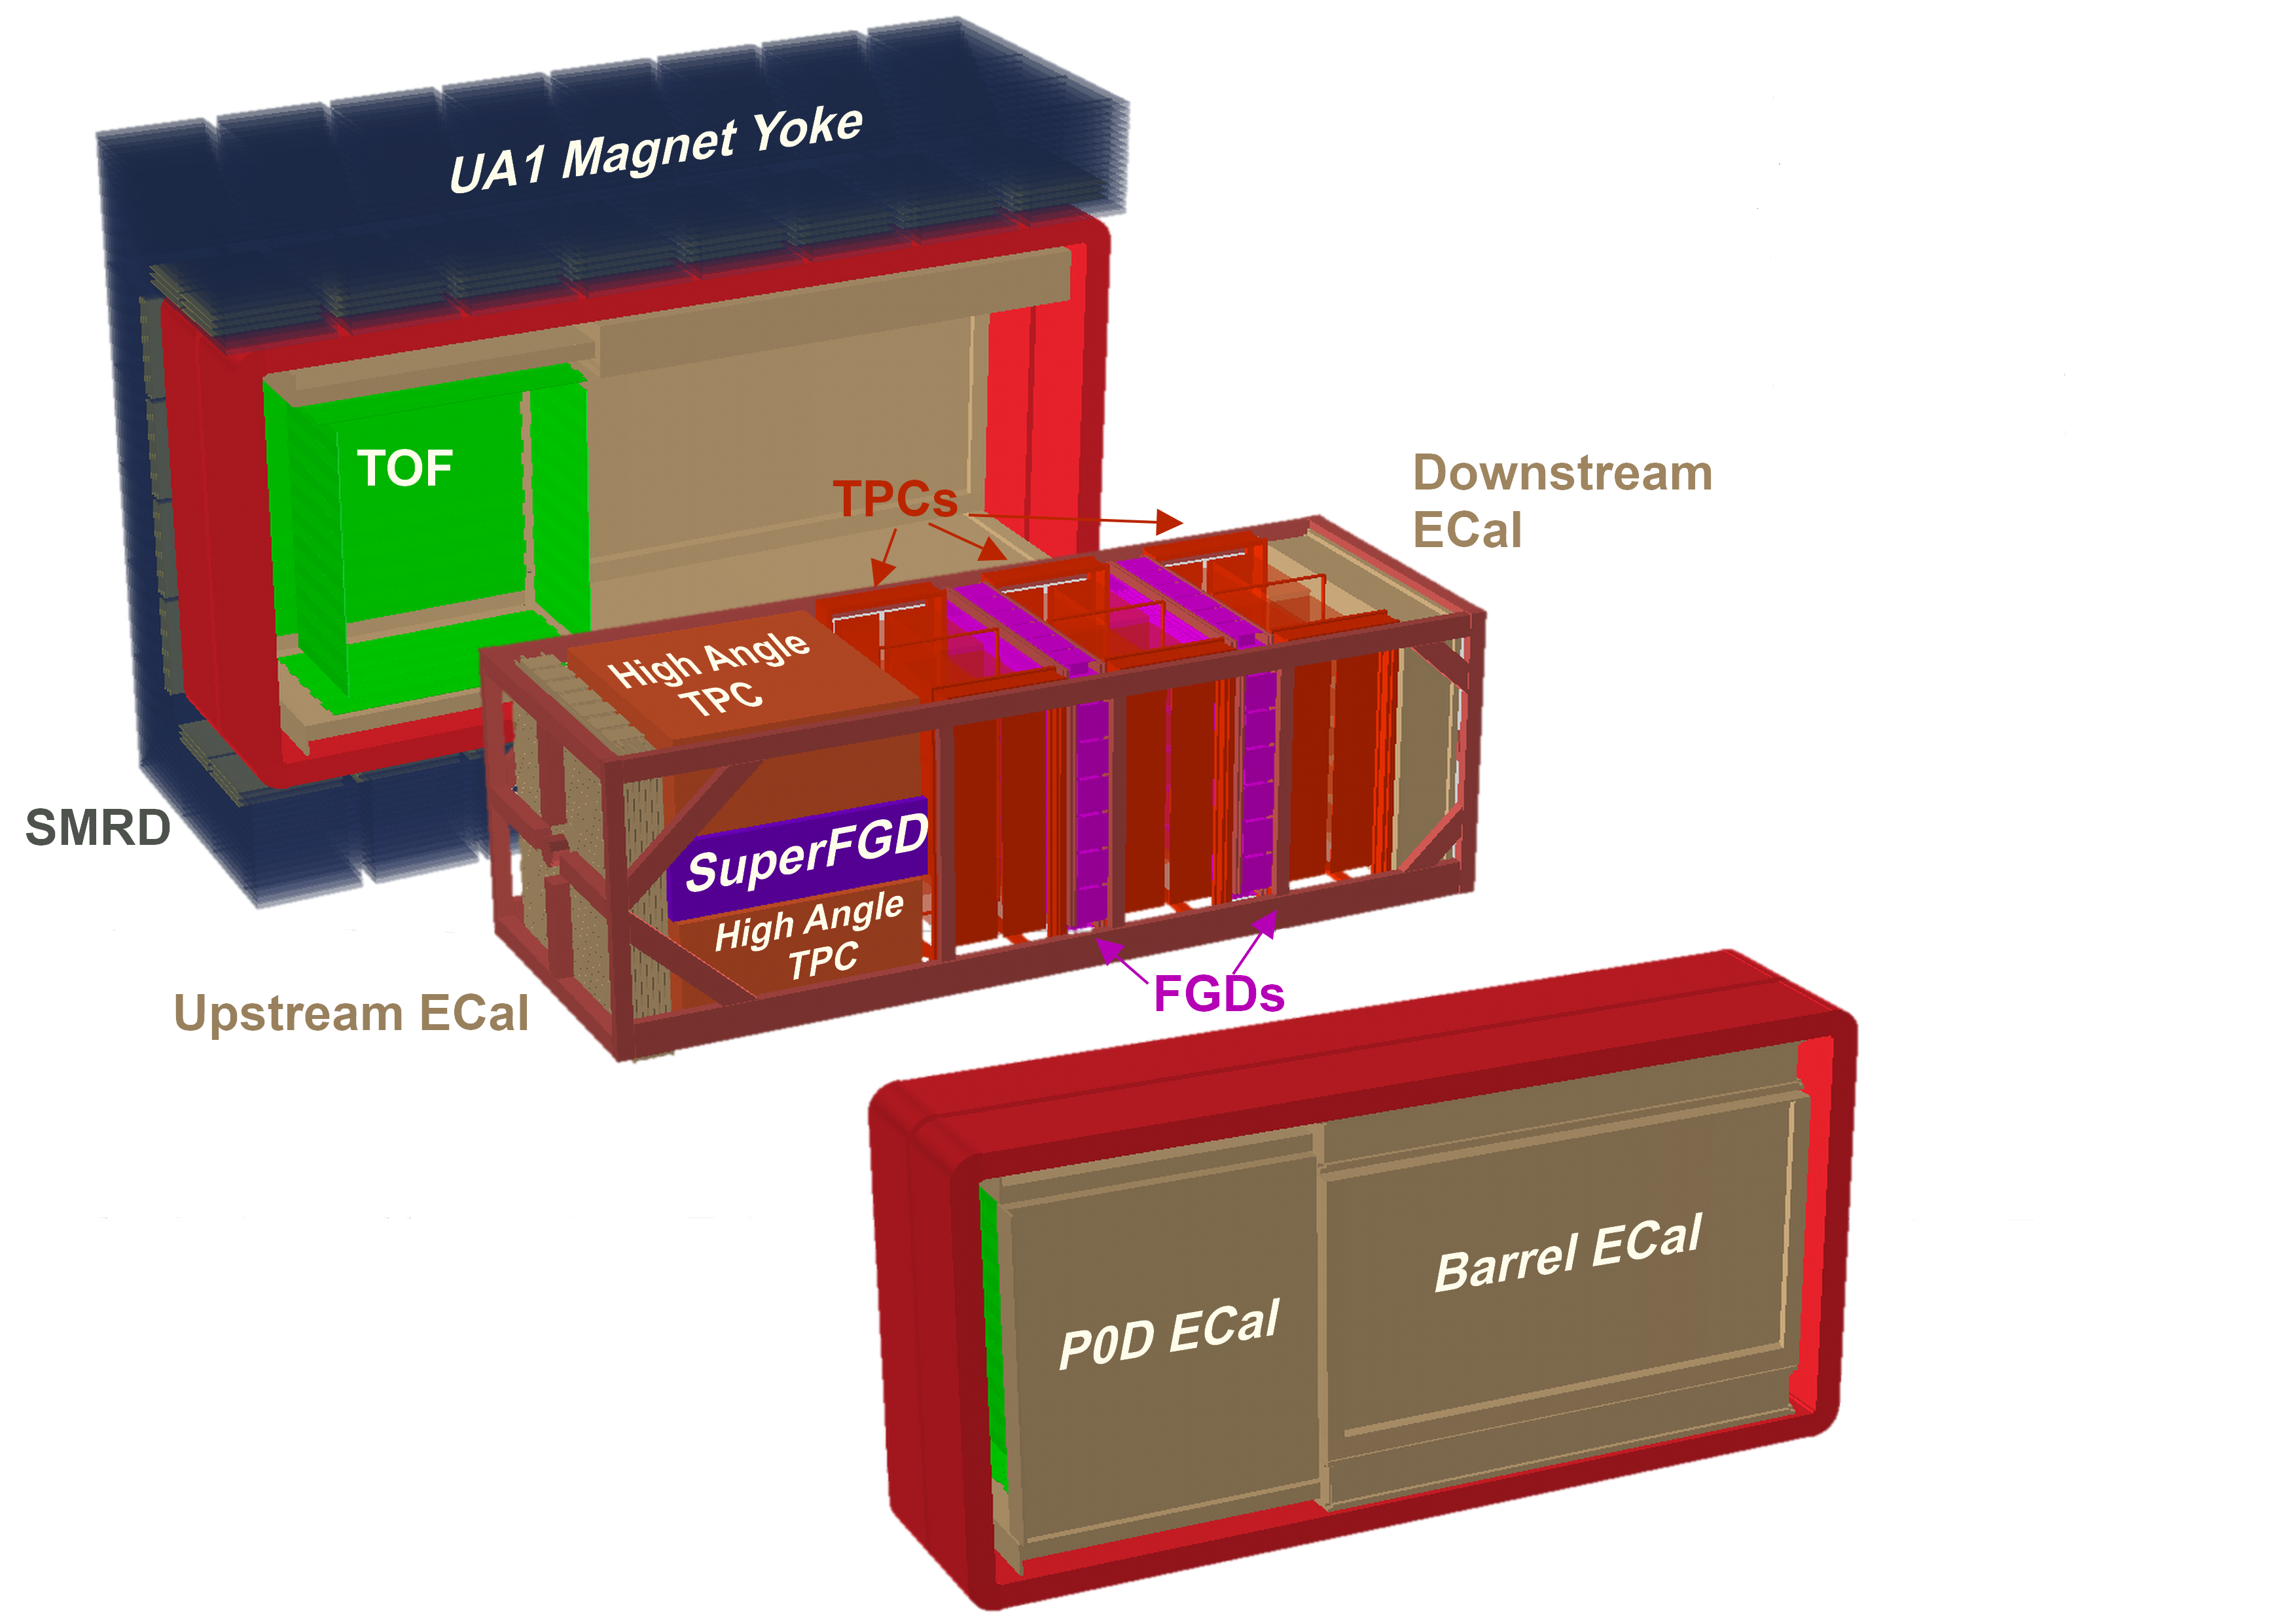
\includegraphics[width=\textwidth]{figures/t2k/ND280-up.png}
        \caption{Upgrade}
        \label{subfig:nd280-up}
    \end{subfigure}
    \caption{ND280 detector diagram.}
    \label{fig:nd280-diagram}
\end{figure}

The neutrino beam passes through the P0D, TPCs, and FGDs.  
Each FGD consists of scintillator bars with a cross section of \(1.0~\mathrm{cm} \times 1.0~\mathrm{cm}\).  
Every layer of bars is oriented orthogonally to the layer above it.  
As a particle traverses these layers, it produces photons in the scintillator; these photons are collected by wavelength-shifting fibers embedded in each bar and ultimately read out by end electronics.  
Hence, the bar recording the signal determines the track position transverse to the neutrino beam, while the layer index specifies the longitudinal position of the energy deposition.

Originally, FGDs served as the active target for neutrino interactions.  
However, their bar geometry offers limited acceptance for particles traveling at large angles to the beam direction—i.e., along the bar’s long axis—because such particles intersect only a few bars, making them difficult to reconstruct.  
At the far detector, the large Cherenkov detector offers near-isotropic acceptance.
This mismatch in phase space between the near and far detectors increases uncertainties in oscillation analyses.  
Moreover, having sparse signals along the particle trajectory degrades reconstruction resolution.  
These limitations motivated the ND280 upgrade.

In the upgraded ND280, the \(\piz\)-detector is replaced by several new subsystems (Fig.~\ref{subfig:nd280-up}): the Time-of-Flight detector (TOF), two High-Angle TPCs (HATs), and the Super Fine Grained Detector (SFGD).  
The TOF comprises six layers of scintillator bars with sub-nanosecond timing resolution, which help veto crossing particles and enhance sample purity.  
The HATs incorporate a redesigned field cage and new Micromegas detectors, expanding the tracking volume and improving resolution relative to the original vertical TPCs.  
Serving as the new active target, the SFGD consists of about two million \(1\,\mathrm{cm}^3\) scintillator cubes.  
Its finer segmentation markedly increases acceptance for high-angle tracks, better aligning with the near-isotropic acceptance at the far detector.  
Additionally, the improved tracking, enabled by enhanced energy deposition measurements, lowers detection thresholds and sharpens resolution, facilitating new reconstruction strategies (e.g., trackless pion reconstruction) and innovative variables (e.g., center-of-mass variables), which will be introduced in the subsequent chapters.  
Construction for the upgrade was completed in April 2024, and data taking with the upgraded ND280 commenced in June 2024.

\section{Software}
\label{sec:t2k-sw}
This thesis focuses primarily on improving reconstruction performance; thus, the following overview of the software used for ND280’s upgraded system aims to clarify and contextualize the methodologies employed in later chapters.

Each scintillator cube in the SFGD contains three passing optical fibers, each is connected to electronics at one of the ends. 
As a charged particle traverses these cubes, scintillation photons travelled along the optical fibers and are measured by readout boards located on three orthogonal faces of the SFGD.  
After calibration, these signals are digitized and assembled into three-dimensional “Hits,” each corresponding to a specific cube position and including a measure of the deposited charge.  
The reconstruction software then sorts these Hits into either clusters or tracks using clustering and track-fitting algorithms.  
Clusters consist of fewer than three Hits, whereas tracks typically contain many more, becasue objects containing too fews Hits are not long enough to be considered as tracks. 
Additionally, due to imperfect optical isolation between cubes, light may leak into neighboring cubes not traversed by the particle.  
To account for this, the reconstruction merges nearby Hits into “Nodes,” which more accurately capture the particle’s trajectory.  
Energy deposition at each Node is then estimated from the associated Hits and refined according to the expected continuous energy loss along the path.  
Finally, a Boosted Decision Tree (BDT), trained on Particle Gun simulations, uses these smoothed energy values and other measured parameters for particle identification and momentum estimation.  